\newpage
\section{L'environement du stage}
L'environement de travail d'un stage dans un laboratoire de recherche est sans doute très différent d'un stage plus classique dans une entreprise privé. En effet, un laboratoire de recherche s'inscrit dans une organisation complexe et possède de nombreuses relations avec d'autres organisations ou d'autres personnes.

Dans cette partie nous présenterons tout d'abord ce qu'est le Laboratoire de l'Informatique du Parallélisme ainsi que ces relations avec d'autres institution, ensuite nous présenterons l'équipe AVALON dont je fais partie, et enfin nous terminerons par présenter la place que j'occupe au sein du laboratoire.

\subsection{Le laboratoire et ses relations institutionnelles}
Le Laboratoire de l'Informatique du Parallélisme (abrégé \gls{lip}) est un laboratoire de recherche en informatique situé principalement sur le site Monod de l'École Normale Supérieure de Lyon.

\subsubsection{Présentation générale}
Créé dans les années 80, le Laboratoire de L'Informatique du Parallélisme devient \gls{ura} (URA) de l'\gls{ens} Lyon en 1989, puis \gls{umr} (UMR) en 1999 qui sera complété par l'Université Claude Bernard Lyon 1 en 2003. Le laboratoire est très tôt épaulé par l'Institut national de recherche en informatique et en automatique (\gls{inria}) qui est le principal acteur de la recherche en informatique et mathématique en France depuis 1967. Ainsi le laboratoire héberge plusieurs équipes-projets communes avec l'\gls{inria}. \cite{reportHCERES}\\

Le laboratoire compte 57 enseignant titulaires et chercheurs, entre 40 et 50 doctorants ainsi qu'une vingtaine de personnes sur des postes non permanents. L'équipe d'administration et l'équipe technique quant-à-elles sont épaulés par 12 ingénieurs.\\

Le \gls{lip} possède une bonne visibilité de ses équipes au niveau national et de plusieurs de ses membres au niveau international. Il occupe une place central dans le paysage de la recherche en informatique français pour quasiment l'ensemble de ses thématiques. La forte croissance du laboratoire lui a même obligé a s'étendre sur 2 autres sites : au sein de l’Institut Rhône-Alpin des Systèmes Complexes, et au sein de locaux appartenant à l’UCB à Gerland.

\subsubsection{Organisation générale}
Le laboratoire compose l'\gls{umr} 5668 avec l'ENS Lyon (EnsL), l'Université Claude Bernard Lyon 1, l'\gls{inria} et le CNRS. Il est dirigé par \textbf{M. Patrick Baillot} qui est secondé par \textbf{M. Frédéric Vivien}. Le responsable en charge de l'appel à projets, de la valorisation de recherche et des relations internationales est \textbf{M. Eddy Caron} et le responsable en charge des thèses, de l'enseignement et des postes non permanents est \textbf{M. Damien Stehlé}.

L'équipe administrative et l'équipe en charge des moyens informatique quant-à-elles sont composés de différentes personne issues des institutions qui constituent l'\gls{umr} 5668.\\

Le laboratoire héberge sept équipes de recherche dont cinq sont commune avec l'\gls{inria} : AriC, Avalon, CASH, DANTE, MC2, PLUME et ROMA chacune administrés par un chef d'équipe.

\begin{figure}[h]
	\center
	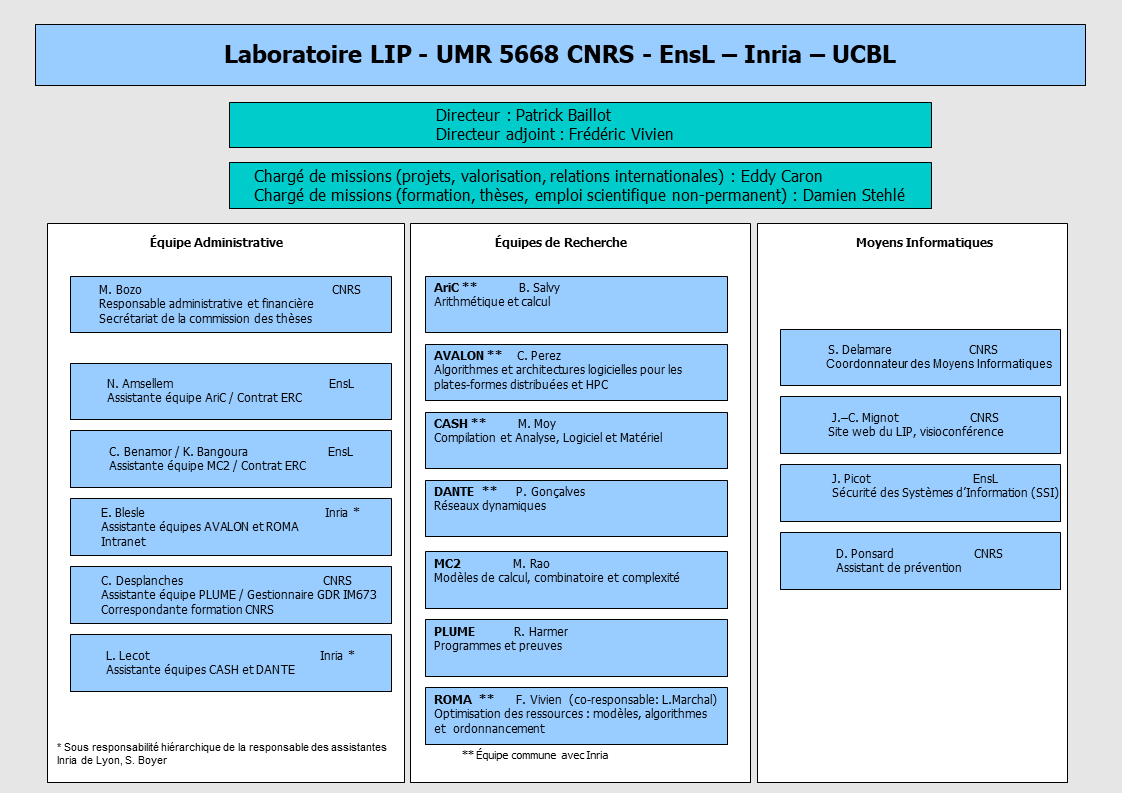
\includegraphics[scale=0.58]{partie1/images/organigramme.png}
	\caption{Organigramme du LIP au 10 Avril 2018 \cite{organigramme}}
\end{figure}
\subsubsection{Des métiers variés}
Le projet du Laboratoire de l'Informatique du Parallélisme est de mettre en relation l'informatique fondamental et sa mise en œuvre pratique dans les institutions. Ainsi le laboratoire crée un lien fort entre informatique et d'autres sciences comme les mathématiques, les sciences du vivant ou, plus globalement, les sciences fondamentales.\cite{presUCBL}\\

Les chercheurs du \gls{lip} possèdent un socle commun : l'algorithmie et l'utilisation efficace des ressources. Ils organisent leurs recherches autour de deux grands axes :
\begin{itemize}
	\item La conception, l'utilisation et l'adéquation aux besoins des applications des futurs architectures de calcul (traitement de données, calcul fondamental) et de communication (réseaux)
	\item L'étude des modèles et des méthodes en informatique : compléxité, algorithmie, développement logiciel et matériel, avancée technologiques etc.\\
\end{itemize}

Ainsi, le laboratoire ne compte pas dans ses rang uniquement des expert de l'informatique. D'autres profils bien différents sont mis en valeurs dans les 7 équipes-projets que nous allons présenter.
\newpage

\textbf{AriC - Arithmetic and Computing}\\
AriC est une grande équipe projet commune avec l'\gls{inria} composée d'une vingtaine de membres. Elle à pour but d'améliorer le calcul, en terme de performance, d'efficacité et de fiabilité. Ses 3 principaux projets de recherche portent sur les sujets suivants :
\begin{itemize}
	\item Les réseaux euclidiens : algorithme et cryptologie,
	\item Les méthodes d'approximation efficaces en calcul formel,
	\item Le calcul fiable à haute performance, avec virgule flottante et précision d'au plus une centaine de bits.
\end{itemize}
Au delà de la recherche cette équipe à une véritable vocation à la diffusion et à la vulgarisation de leurs travaux, ce qui passe par la multiplication des interventions dans les lycées ou autre institutions d'enseignement et la publication d'articles et d'ouvrages \cite{aric}.\\

\textbf{Avalon - Algorithms and Software Architectures for Distributed and HPC Platforms}\\
L'objectif de l'équipe commune \gls{inria} Avalon est de concevoir des modèles de programmations, des systèmes et des algorithmes pour exécuter des applications sur des ressources tout en satisfaisant les contraintes des utilisateurs (e.g.\ coût, performances) et des administrateurs (e.g.\ maximisé l'usage des ressource, minimiser la consommation d'énergie).
L'équipe se concentre en particulier sur le profilage et la modélisation d'applications gourmandes en énergie et en données, la gestion des données et l'ordonnancement des applications sur des architectures de supercalculateurs \cite{avalon}.\\

\textbf{CASH - Compilation and Analyses for Software and Hardware}\\
La vision de l'équipe commune \gls{inria} CASH est d'utiliser l'architecture \gls{dataflow} pour le traitement des données par les supercalculateurs. Son but est d'utiliser les caractéristiques particuliers du matériel informatique afin de fournir des couples matériel-logiciel efficaces énergétiquement au développeur final. Pour ce faire elle travaille sur les axes d'études suivants :
\begin{itemize}
	\item Développer l'architecture \gls{dataflow},
	\item Améliorer les algorithmes de compilation,
	\item Développer la compilation matériel, qui consiste à transformer un programme informatique en un circuit électronique physique,
	\item Émuler les \glspl{systemepuce} pour faciliter leur optimisation \cite{cash}.\\
\end{itemize}

\textbf{DANTE - Dynamic Network}\\
L'objectif principal de l'équipe commune \gls{inria} DANTE est de poser des bases solides à la caractérisation des réseaux dynamiques et des processus dynamiques se produisant sur des réseaux à grande échelle. Afin de développer des outils d'une pertinence pratique en situation réelle, elle fonde ses études méthodologiques sur des jeux de données réelles. Ses 3 grands thèmes de recherche sont :
\begin{itemize}
	\item Le traitement du signal basé sur les graphes,
	\item La théorie des graphes dynamiques,
	\item Les \glspl{algodistrib} pour les réseaux dynamiques \cite{dante}.
\end{itemize}
\newpage
\textbf{MC2 - Models of computation, Complexity, Combinatorics}\\
L'équipe MC2 à pour but de comprendre les possibilités et les limitations des algorithmes efficace. Pour ce faire elle crée et analyse des algorithme jusqu'à leurs limites. Parmi les différents domaines des mathématiques au cœur de ses problématiques, l'équipe MC2 se concentre sur l'algèbre et l'\gls{analysecombinatoire}. Ces deux domaines sont des sources de problèmes algorithmiques qui jouent un rôle clé dans la théorie de la \gls{complexite} \cite{mc2}.\\

\textbf{PLUME - Programs and Proof}\\
Les recherches menées par l'équipe PLUME s'articulent autour de deux thèmes fortement imbriqués : les fondements logiques des langages de programmation et la théorie des systèmes informatiques. Elle met au centre de ses recherche la logique mathématique afin de trouver comment écrire des programmes sûrs ou comment vérifier formellement des systèmes informatique complexes \cite{plume}.\\

\textbf{ROMA - Resource Optimization : Models, Algorithms and Scheduling}\\
L'équipe commune \gls{inria} ROMA vise à concevoir des modèles, des algorithmes et des stratégies d'ordonnancement pour optimiser l'exécution d'applications scientifiques sur des supercalculateurs. Plus spécifiquement, ROMA vise à obtenir la "meilleure" performance possible du point de vue de l'utilisateur (e.g.\ le temps d'exécution de l'application) tout en utilisant les ressources aussi efficacement que possible \cite{roma}.\\

Ainsi, le Laboratoire de l'Informatique du Parallélisme possède un impressionnant savoir faire dans de nombreux domaines de l'informatique et produit de nombreuses ressources pour des institutions publiques et privés, comme nous allons le voir.

\subsubsection{Une production conséquente}
Le Laboratoire de l'Informatique du Parallélisme est plutôt prolifique dans la quantité de production. Depuis 2000, 2502 publications ont été publiés et sont disponibles sur des plateforme en ligne comme les archives ouvertes HAL. En effet le laboratoire est dans une véritable démarche de production de connaissances, mais cela ne l'empêche pas de s'autofinancer grâce à des contrats industriels et des projets institutionnels régionaux, nationaux et internationaux \cite{reportHCERES}. 2 brevets ont même été déposés.\\

Le laboratoire encourage également les ambitions d'entrepreneuriat de ses membres avec la création de 5 start-ups dans le domaine du numérique depuis 2010 \cite{presUCBL}.\\

Enfin, les différentes équipes du laboratoire produisent également de nombreuses ressources logicielles open-source à destinations des institutions, les industriels et même des particuliers que l'on peut retrouver sur les plateforme de partage de code source en ligne.
\subsection{L'équipe Avalon en détails}
L'équipe dont je fais parti durant ce stage est l'équipe Avalon. Cette équipe créée le 1er Février 2012 \cite{avalonAR2012} est une équipe-projet du Laboratoire de l'Informatique du Parallélisme commune à l'\gls{inria} et composée de 22 membres : 8 universitaires permanents, 2 universitaires temporaires, 4 membres permanents et 8 doctorants. Elle est située au troisième étage de l'aile sud du bâtiment M7 sur le site Monod de l'École Normale Supérieure de Lyon.

\subsubsection{Les membres de l'équipe}
Parmi les 22 membres de l'équipe, voici un rapide aperçu de ceux que j'ai côtoyé durant mon stage :\\

\textbf{Universitaires permanents}
\begin{figure}[h!]
   \begin{minipage}{0.33\textwidth}
		\centering
		
\includegraphics[height=3cm]{partie1/images/christian.jpg}\\
		\textbf{Christian Perez}\\
		Chef de l'équipe\\Chercheur sénior Inria
	\end{minipage}\hfill
	\begin{minipage}{0.33\textwidth}
		\centering
		
\includegraphics[width=3cm]{partie1/images/eddy.jpeg}\\
		\textbf{Eddy Carron}\\
		Responsable administratif\\Enseignant chercheur
	\end{minipage}\hfill
	\begin{minipage}{0.33\textwidth}
		\centering
		
\includegraphics[width=3cm]{partie1/images/laurent.jpg}\\
		\textbf{Laurent Lefèvre}\\
		Mon maître de stage\\Chercheur Inria
	\end{minipage}
\end{figure}

\textbf{Universitaires temporaires}
\begin{figure}[h!]
	\begin{minipage}{0.48\textwidth}
		\centering
		
\includegraphics[height=3cm]{partie1/images/marco.jpg}\\
		\textbf{Marcos Dias de Assuncao}\\
		Chercheur
	\end{minipage}\hfill
	\begin{minipage}{0.48\textwidth}
		\centering
		
\includegraphics[height=3cm]{partie1/images/cyril.jpg}\\
		\textbf{Cyril Seguin}\\
		Chercheur PostDoc\\Expert Cloud et Sécurité
	\end{minipage}\hfill
\end{figure}

\textbf{Équipe}
\begin{figure}[h!]
	\begin{minipage}{0.33\textwidth}
		\centering
		
\includegraphics[height=3cm]{partie1/images/evelyne.jpeg}\\
		\textbf{Evelyne Blesle}\\
		Assistante administrative
	\end{minipage}\hfill
	\begin{minipage}{0.33\textwidth}
		\centering
		
\includegraphics[width=3cm]{partie1/images/simon.jpeg}\\
		\textbf{Simon Delamare}\\
		Ingénieur de recherche
	\end{minipage}\hfill
	\begin{minipage}{0.33\textwidth}
		\centering
		
\includegraphics[width=3cm]{partie1/images/matthieu.jpeg}\\
		\textbf{Matthieu Imbert}\\
		Ingénieur de recherche
	\end{minipage}
\end{figure}
\newpage
\textbf{Doctorants}
\begin{figure}[h!]
	\begin{minipage}{0.33\textwidth}
		\centering
		
\includegraphics[height=3cm]{partie1/images/issam.jpeg}\\
		\textbf{Issam Raïs}\\
		Thèse sur l'étude de la consommation énergétique des supercalculateurs
	\end{minipage}\hfill
	\begin{minipage}{0.33\textwidth}
		\centering
		
\includegraphics[width=3cm]{partie1/images/dorra.png}\\
		\textbf{Dorra Boughzala}\\
		Thèse sur la simulation de la consommation d'énergie des architecture hétérogènes
	\end{minipage}\hfill
	\begin{minipage}{0.33\textwidth}
		\centering
		
\includegraphics[width=3cm]{partie1/images/alexandre.jpg}\\
		\textbf{Alexandre da Silva Veith}\\
		Thèse sur les algorithmes pour l'analyse des flux élastiques du Big-Data
	\end{minipage}
\end{figure}
\begin{figure}[h!]
	\begin{minipage}{0.33\textwidth}
		\centering
		
\includegraphics[height=3cm]{partie1/images/hadrien.jpeg}\\
		\textbf{Hadrien Croubois}\\
		Spécialisé dans les processus parallèles et les systèmes distribués
	\end{minipage}\hfill
	\begin{minipage}{0.33\textwidth}
		\centering
		
\includegraphics[width=3cm]{partie1/images/felipe.jpg}\\
		\textbf{Felipe Rodrigo de Souza}\\
		Thèse sur les algorithmes de provisionnement des réseaux
	\end{minipage}\hfill
	\begin{minipage}{0.33\textwidth}
		\centering
		
\includegraphics[width=3cm]{partie1/images/valentin.jpg}\\
		\textbf{Valentin Lorentz}\\
		Thèse sur la traçabilité énergétique des données
	\end{minipage}
\end{figure}

\subsubsection{Le contexte de création}
Formée le 1 Février 2012, l'équipe Avalon est une véritable réponse aux changements effrénés de l'informatique.
L'évolution très rapide du matériel informatique en terme de communication, de traitement de données et de virtualisation a fait émerger des nouveaux besoins pour l'utilisateur. En effet la complexité des systèmes informatiques augmente !
Il existe aujourd'hui de nombreuses variétés de plateformes à grande échelle disponibles pour des chercheurs ou des industriels qui souhaitent satisfaire leurs besoins en traitement de données : agrégation de \glspl{cluster}, grand \glspl{datacenter}, supercalculateurs etc.
Chacune de ces plateformes dispose de spécificités intrinsèques, d'accès et d'utilisation qui ont un impact important sur l'architecture et l'exécution des applications qui souhaitent les utiliser.
Elles intègrent de nombreuses fonctionnalités obligatoires comme le sécurité, la virtualisation, le \gls{load-balancing} ou autres qui augmentent encore plus leur complexité d'utilisation.
C'est dans ce contexte que l'équipe Avalon a été créée, la réponse qu'elle apporte est d'aller plus loin dans l'abstraction de ces plateformes pour assurer à l'utilisateur une utilisation simplifiée tout en gardant l'ensemble des fonctionnalités disponibles. \cite{avalonAR2012}

\subsubsection{La vision de l'équipe}
La vision de l'équipe Avalon est de considérer l'ensemble du système, de la ressource à l'application, afin de concevoir des outils simples à utiliser par les programmeurs tout en permettant une exploitation efficace des ressources.
L'équipe se concentre en particulier sur la gestion de l'élasticité (i.e\ la capacité à s'adapter aux besoins des applications le plus rapidement possible) des plateforme parallèles et distribués ainsi que leur efficacité énergétique. \cite{avalonAR2012}\\

L'équipe souhaite pouvoir mettre à disposition d'autres équipes de recherche travaillant dans d'autres sciences des ressources informatiques à haute performance de manière simple à utiliser.

Voici quelques exemples de disciplines qui pourrait avoir recours aux travaux de l'équipe Avalon :
\begin{itemize}
	\item La biologie, avec par exemple le séquençage de l'ADN,
	\item L'étude du climat, qui demande une quantité de paramètres impressionnante pour simuler les changements de climat prochains,
	\item L'astrophysique, qui est demandeuse de simulations pour comprendre les phénomènes physique qui nous entoure, la formation des galaxies, pour étudier la matière noire etc.
\end{itemize}
\subsection{Mon environement au sein du laboratoire}
Dans cette partie nous allons voir dans quel environement de travail j'ai évolué tout au long de mon stage au sein du laboratoire. Nous présenterons tout d'abord comment s'est organisé le travail, ensuite dans quel environement technique j'ai évolué et enfin quelles sont mes interactions avec les autres membres de l'équipe.

\subsubsection{Les horaires de travail}
Le travail au laboratoire est assez librement organisé. En effet, pendant toute ma période de stage j'ai eu, dans la limite d'effectuer 35 heures par semaines, des horaires libres. Cela m'a permis d'organiser facilement d'autres tâches importantes de cette période, notamment les entretiens avec les écoles d'ingénieurs pour mon admission en alternance, le forum d'entreprise obligatoire de Polytech ou encore mes entretiens individuels avec des entreprises dans le but de dénicher un contrat d'apprentissage.\\

Contrairement à lorsque j'étudiais à l'IUT où j'aurais farouchement défendu ma pause de midi de 2h ainsi que mes pauses de 20 minutes toutes les deux heures, je n'ai pas spécialement ressenti pendant ce stage le besoin de prendre de longues pauses. C'est pour cela, qu'après quelques jours, je me suis basé sur un rythme de travail de 9h--16h30.\\

Arriver à 9h est déjà une grande différence par rapport à l'IUT, c'est tout d'abord une heure plus tard, mais mon temps de trajet étant également plus court pour aller au laboratoire que pour aller à l'IUT, cela me permet de me lever 1h20 plus tard tous les matins.\\

Pour le temps de midi, une petite particularité du laboratoire est qu'il utilise pour manger le restaurant universitaire de l'ENS Lyon, ainsi pour ne pas faire la queue, les équipes ont décidés de descendre manger à 11h30. Tous les midis une partie de l'équipe Avalon descend ensemble manger pendent environs 30 minutes, puis remonte. Il reste alors 4h30 de travail pour arriver aux 7 heures de travail quotidien.\\

Je me suis fais la réflexion que ce rythme de travail n'est peut-être pas le plus adéquat en raison de son déséquilibre entre le temps de travail du matin et de l'après midi. Mais je n'étais pas convaincu par le fait d'arriver à 8h et de repartir à 15h30.
 
\subsubsection{Les locaux}
Ce stage s'est déroulé dans les locaux du LIP, au troisième étage du bâtiment M7 du site Monod de l'ENS Lyon. Pratiquement tous les membres de l'équipe Avalon sont situés au même endroit : un grand couloir dessert de part et d'autres des bureaux de deux, parfois trois, personnes.\\

Au début de mon stage j'étais situé dans le dernier bureau du couloir que je partageais avec \textbf{Issam Raïs}, doctorant sous la supervision de mon maître de stage Laurent Lefèvre. Le 22 mai, une réorganisation des bureaux a été faites, j'ai quitté Issam pour rejoindre, dans le bureau situé juste avant, \textbf{Lucas Besnard}, un camarade de promotion qui effectue également son stage au LIP, mais qui ne travaille pas sur le même sujet que moi.\\

Les bureaux sont relativement spacieux, possèdent une armoire commune ainsi qu'un casier individuel. Le principale problème est que l'équipe est situé dans l'aile Sud du bâtiment et que les bureaux sont équipés d'une grande baie vitré coté Sud. Lorsqu'il y a du soleil le travail devient très vite difficile en raison des températures. Heureusement nous avions la possibilité de nous réfugier dans la bibliothèque de l'ENS, qui est climatisée, si cela devenait intenable.\\

Le bâtiment possède également des boxs de travail ou nous pouvions nous retrouver pour travailler à plusieurs, ainsi qu'une grande salle de réunion. Après le couloir, un solarium était également à notre disposition avec des transats, qui m'ont bien été utiles lors de la lecture de publications scientifiques.

\subsubsection{L'environement matériel}
Le laboratoire pouvait me fournir un ordinateur portable ainsi qu'une station d'accueil pour effectuer me travaux. Cependant ces machines n'étant pas très performantes on m'a conseillé d'utiliser mon ordinateur personnel.\\

On m'a par contre fourni un deuxième écran, qui est quelque-chose que je trouve de plus en plus indispensable. Il est d'ailleurs tombé en panne quelques semaines plus tard, probablement à cause de la chaleur, mais Issam m'a très gentiment prêté un de ses écrans qu'il n'utilisait pas.

\subsubsection{L'environement technologique}
L'équipe Avalon ne possède pas vraiment d'environement technologique propre, car chaque membre utilise les technologies les plus pertinentes pour chaque tâche. Cependant, elle utilise activement le plateforme \emph{Grid'5000} que je vais présenter.\\

\begin{figure}[h!]
	\centering
	
\includegraphics[width=5.5cm]{partie1/images/grid5000_logo.png}
	\caption{Logo de la plateforme Grid'5000}
\end{figure}

Grid'5000 est un banc d'essai à grand échelle pour la recherche expérimentale en informatique. Cette plateforme met à disposition des chercheurs un très grande quantité de ressources informatiques : plus de 1000 serveurs, 8000 cœurs de processeur regroupés en \glspl{cluster}. Elle est utilisé par une communauté de plus de 500 utilisateurs et est hébergée sur une dizaine de sites en France. \cite{grid5000home}\\

Elle est à la pointe de la technologie avec notamment une connexion au réseau de 10Gbit/s (5000 fois meilleure que la box qui vous connecte à Internet), des connectiques \emph{Infiniband} qui permettent un débit jusqu'à 56Gbits/s ou encore les processeurs ultra performants \emph{Xeon PHI} du constructeur leader \emph{Intel}.\\

La plateforme intègre de nombreux outils de monitoring et de mesure afin de permettre des expérimentations et leurs interprétations très précises. Elle possède notamment un arsenal de Wattmètres qui mesurent au plus près de la machine la consommation du matériel et qui sont beaucoup utilisés par les membres de l'équipe Avalon, notamment par Issam et Dorra pour leurs thèses et mon camarade Lucas pour son stage.\\

Afin de nous former, Lucas et moi, à l'utilisation de cette plateforme nous avons été formé par \textbf{Dorra Boughzala}, qui venait d'effectuer une formation complète. Nous avons passé 2 à 4 heures par jour en sa compagnie pendant la première semaine de notre stage. Je n'avais jamais utilisé une telle plateforme, mais étant déjà familiarisé aux environnements Linux ainsi qu'à certains concepts, j'ai pû assez facilement m'approprier l'outils, qui s'avère extrêmement intéressant et puissant.
 
\subsubsection{L'environement humain}
Évidemment, un laboratoire de recherche est international, un certain nombre des membres de l'équipe ne sont donc pas français. Tout le monde parle bien l'anglais ce qui permet de très bien se comprendre, mais la barrière de la langue se fait parfois ressentir lorsqu'on troque les interactions formelles pour des interactions plus amicales. Les interactions avec les différents membres de l'équipe et du laboratoire sont d'ailleurs très décontractés, tout le monde se tutoie, par exemple.\\

Pour ma mission je ne communiquais qu'avec Laurent, mon maître de stage qui prennait note de l'avancement du projet tout en m'aiguillait et en me proposant des pistes à suivre, parfois en me fournissant des publications scientifiques. Il n'a cependant pas participé à la phase de développement, où j'étais en toute autonomie.

\subsubsection{Les groupes de travail}
Lorsque l'équipe en ressent le besoin, des groupes de travail sont organisés. Toute l'équipe se retrouve ensemble dans une sale de réunion. Souvent elle procède à une \emph{round table}, qui consiste à présenter ce sur quoi on travaille, ce que l'on a fait depuis la dernière \emph{round table} et ce que l'on a prévu de faire pour la suite. Mais parfois il peut s'agir d'un membre de l'équipe qui souhaite présenter, une technologie, son travail ou tout autre chose.\\
Les membres mettent également par écrit ce qu'ils ont dit durant le groupe de travail, ce qui permet à Alexandre de mettre à jour le site internet de l'équipe Avalon.